\documentclass[a4paper,12pt]{article}
\usepackage[french]{babel}
\usepackage[T1]{fontenc}
\usepackage[utf8]{inputenc}
\usepackage{graphicx}
\usepackage{pdfpages}
\usepackage{fancyhdr}
\pagestyle{fancy}
\fancyhead[L]{PAO Nao joue à pong}
\fancyhead[R]{ASI 3.2 - INSA Rouen}
\fancyfoot[L]{GICQUEL - MARTIN - THEOLOGIEN}
\fancyfoot[R]{\thepage}
\fancyfoot[C]{}

\newcommand\theHsubsubsubsection{\theHsubsubsection.\arabic{subsubsubsection}}

\setcounter{secnumdepth}{4}
\setcounter{tocdepth}{3}
\makeatletter
\newcounter {subsubsubsection}[subsubsection]
\renewcommand\thesubsubsubsection{\thesubsubsection .\@arabic\c@subsubsubsection}
\newcommand\subsubsubsection{\@startsection{subsubsubsection}{4}{\z@}%
                                     {-1.25ex\@plus -1ex \@minus -.2ex}%
                                     {1.5ex \@plus .2ex}%
                                     {\normalfont\normalsize\bfseries}}
\newcommand*\l@subsubsubsection{\@dottedtocline{3}{7.0em}{4.1em}}
\newcommand*{\subsubsubsectionmark}[1]{}
\makeatother


\newcommand{\pao}{\textit{Projet d'Approfondissement et d'Ouverture}}
\newcommand{\projet}{\textit{Nao joue à Pong}}


\title{NAO joue à Pong}
\author{
	Enora GICQUEL\\
	Florian MARTIN\\
	Thibault THEOLOGIEN
}

\begin{document}
%	\makeatletter
%	\begin{titlepage}
%		\begin{center}
%			\centering
%
%      {\large \textsc{INSA Rouen}}\\
%      \textsc{Département ASI}\\
%
%			\vspace{2em}
%      {\large \textbf{\@date\\
%       								Rapport de PAO}}\\
%	    \vspace{6em}
%	     {\LARGE \textbf{\@title}} \\
%	    \vfill
%	      {\large \@author} \\
%		\end{center}
%	\end{titlepage}
%	\makeatother

\begin{titlepage}
\thispagestyle{empty}
\begin{figure}
	\includegraphics[width=5cm]{Images/Insa.png}\hfill
	\includegraphics[width=5cm]{Images/ASI.png}\
\end{figure}

\newcommand{\HRule}{\rule{\linewidth}{0.5mm}} 
\center 
\vspace*{\stretch{1}}\textsc{\huge Institut National des Sciences Appliqu\'{e}es de Rouen}\\[1.5cm] 
\textsc{\Large Projet d'Approfondissment et d'Ouverture}\\[2cm] 

\HRule \\[0.4cm]
{ \huge \bfseries Nao joue à Pong}\\[0.2cm] 
\HRule \\[2.5cm]
  


\large \emph{\textbf{Auteurs :}}\\
	Enora GICQUEL\\
	Florian MARTIN\\
	Thibault THEOLOGIEN \\

~\\ ~\\[1cm]

\vfill{\today}\\[3cm]

\end{titlepage}

	\pagebreak
	\tableofcontents
	\pagebreak

	\section{Introduction}
\label{sec:Introduction}

\par Lors de ce semestre d'ASI 3.2, nous avions la possibilité de suivre un \pao.
Nous avons repris le sujet \projet\ qui a débuté au semestre précédent sous la direction de Monsieur Nicolas Delestre.

\par Nous avons choisi ce sujet afin d'appliquer nos compétences en développement informatique dans un contexte nouveau, à savoir la robotique.
Nous étions également intéressés par la découverte d'outils de programmation pour une utilisation assez ludique.

\par Ce rapport présente l'évolution du projet au cours de ce semestre.
Nous commencerons par analyser le projet tel que nous l'avons repris, pour ensuite présenter nos objectifs pour cette succession.
Nous évoquerons la conception relative au sujet puis son développement. Nous détaillerons aussi les problèmes rencontrés tout au long de la réalisation du projet.
Nous nous attarderons également sur les évolutions possibles en cas de reprise du sujet.
Et nous finirons sur l'évocation des différentes présentations que nous avons pu faire dans le cadre du projet.

\pagebreak

	\section{Etude de l'existant}
\label{sec:Etude de l'existant}
\par Nous avons eu comme base le code produit par une équipe auparavant qui avait pour 
but de produire une version permettant de confirmer la faisabilité du projet. Leur travail 
s'articulait autour de deux grands points qui sont l'IA et principalement la reconnaissance.

    \subsection{Reconnaissance}
    \par L'équipe précédente a produit différents modules de 
    reconnaissance. Ainsi ces différentes méthodes allaient de la comparaison d'histogramme, 
    qui se trouvait être peu fonctionnelle et offrait trop souvent de faux positifs au niveau 
    de la reconnaissance. Une autre méthode qui a été celle retenue consistait en l'utilisation 
    de la bibliothèque OpenCV, spécialisée dans le traitement d'images en temps réel, afin de 
    trouver les contours et formes des images afin de détecter les différents éléments du jeu de Pong.
    
    \par Cette méthode retenue offrait la plupart du temps une bonne reconnaissance du terrain,
    ainsi que des différents éléments du jeu de Pong, mais avait pour défaut majeur un très long 
    temps de traitement. Ainsi, la contrainte de réaction en temps réel du robot pour pouvoir jouer 
    correctement ne pouvait pas être respectée, le traitement durant environ 2 à 3 secondes pour réagir.
    
    \subsection{IA}
    \par L'IA qui a tout d'abord été implémentée était très basique. En effet cette dernière se contentait 
    de suivre la balle sur l'axe vertical avec la raquette. De plus la prise en compte du temps pour atteindre 
    la même hauteur que la balle n'était pas présente, le Nao se contentait donc de se déplacer par accoups afin 
    d'atteindre la position voulue après plusieurs reconnaissances effectuées.
    
    \par Malheureusement, du fait de la lenteur de la reconnaissance, cette solution n'était pas viable 
    pour faire jouer correctement le robot au Pong. Il arrivait donc assez peu souvent que le Nao arrive à 
    atteindre la balle à temps.
    
    \subsection{Structure globale du code}
    \par Le but étant de produire une version permettant de confirmer la faisabilité du projet, 
    le code produit ne suivait pas une structure modulaire, était difficilement maintenable et 
    compréhensible dans l'état dans lequel il se trouvait. Ainsi, les différents appels au robot 
    étaient effectués autant au niveau de l'IA que de la reconnaissance, ce qui rendait le code 
    très difficilement débuggable du fait de la dispersion des traitements dans les différentes 
    parties du code.
    
    \par Nous trouvions donc trois fichiers principaux qui étaient les fichiers \textit{Controle}, \textit{IA} et \textit{Reconnaissance}.

\pagebreak

	\section{Presentation du projet}
\label{sec:Presentation du projet}

\pagebreak

	\section{Conception}
\label{sec:Conception}

\par La conception inhérente au projet à été l'un des points les plus importants pour nous au cours de ce PAO. En effet, notre but étant de fournir un code bien organisé, propre et fonctionnel, il a été important de privilégier la création de diagrammes nous permettant de nous donner une vue d'ensemble du projet.
\par Ainsi deux diagrammes ont étés produits. Tout d'abord un diagramme de classes (annexe \ref{sec:Diagramme de classes} page \pageref{sec:Diagramme de classes}) présentant la répartition du code d'un point de vue axé objet contrairement à ce qui avait été produit précédemment. Et un diagramme de séquence (annexe \ref{sec:Diagramme de séquence} page \pageref{sec:Diagramme de séquence}) présentant le déroulement que nous voulions intégrer au programme principal du projet (Main).
\par Le diagramme de classes s'est vu révisé plusieurs fois afin de s'assurer de la conformité selon la norme UML ainsi que de la logique nécessaire au bon fonctionnement du programme final.
\par Le diagramme de séquence quand à lui, comme dis précédemment, à été produit seulement afin de réfléchir sur ce que devait effectuer le programme en accord avec le diagramme de classes.


	\section{Développement}
\label{sec:Développement}

\pagebreak

	\section{Présentation du projet à des élèves extérieurs}
\label{sec:Présentation du projet à des élèves extérieurs}
  \par Au cours des deux derniers mois du \pao\ nous avons eu l'occasion de présenter à deux reprises notre projet devant des élèves extérieurs.\\

  \subsection{Présentation du 22 avril}
  \label{sub:Présentation du 22 avril}
    \par La première présentation a eu lieu face à des élèves de seconde visitant l'établissement.
    Pour l'occasion, un diaporama expliquant rapidement et de la manière la plus simple le but de notre travail a été conçu.\\
    Nous avons fait le choix d'utiliser le framework JavaScript Reveal.js, pour ce diaporama. 
    Ce framework permet de faire des presentations interactives de manière relativement aisée en HTML / CSS, puis de les visualiser depuis son navigateur. Cependant comme nous ne l’avions pas utilisé depuis un moment, cela a nécessité un certain temps de réadaptation.
    L'avantage de cette solution est qu'elle nous permettait d'utiliser un dépôt git, facilitant la mise en commun et les mises à jour de notre travail.\\
    Trouver comment aborder le sujet du projet pour la présentation devant les lycéens et essayer d’adapter son discours en conséquence n’a pas été si aisé.
    De plus, une démonstration du NAO jouant à pong était requise.
    Cependant, à la date de la présentation, le projet était encore loin de son résultat final, et le code que nous avions ne nous permettait pas de faire une démonstration convenable de notre travail.
    Nous avons donc été contraint de réutiliser le travail effectué par les élèves travaillant avant nous sur ce PAO.\\

  \subsection{Présentation du 10 mai}
  \label{sub:Présentation du 10 mai}
    \par La seconde présentation s'est déroulée devant des élèves en CM1/CM2. \\
    Dans le cadre d'un projet personnel (Chimie Kids) des étudiants en CFI3 nous ont contacté afin que nous leur présentions le département ASI ainsi que notre PAO.
    Cette présentation étant de courte durée et face à d'aussi jeunes élèves, aucun diaporama n'était requis. Nous avons quand même dû donner quelques explications et il se trouve qu'adapter notre discours pour les écoliers s'est révéler encore plus difficile que lors de la présentation face aux lycéens.
    Nous avons également dû effectuer une démonstration du NAO jouant à pong.
    Cette fois, notre avancement dans le projet nous a permis d'utiliser notre code.
\pagebreak

	\section{Problèmes rencontrés}
\label{sec:Problèmes rencontrés}

  \par Au cours de ce projet nous nous sommes retrouvé face à un certain nombre de difficultés, dans des domaines assez variés compte tenu de l'évolution du projet.
  En effet, les problèmes que nous avons pu rencontrer au cours des premières semaines concernaient plus des problèmes matériels,
  tandis que ceux rencontrés durant les dernières semaines étaient plus de l'ordre de contraintes de développement.\\
  Les sous-parties suivantes traiterons donc, par ordre chronologique, de ces problèmes auxquels nous avons dû faire face, ou que nous avons simplement indentifiés.\\

  \subsection{Semaines du 18 janvier au 1 fevrier}
    \label{sub:Semaines du 18 janvier au 1 fevrier}
    \begin{itemize}
      \item Les dépendances du projet ne nous ayant pas été fournies, nous avons dû les récupérer directement depuis internet.
      Or l'API NaoQI, indispensable pour interagir avec le robot, necessite l'obtention d'un statut de développeur au sein de la plateforme aldebaran, statut qui nous a été assez difficile à obtenir.
      \item Nous avons mis un certain temps à nous appercevoir que l'API NaoQI repose sur une ancienne version du langage Python (2.7).
      % NOTE: Flo t'as certainement un truc à ajouter ici pour les contraintes que ça a pu apporter
      \item Le code fourni n'était pas fonctionnel: il contenait un certain nombre de bugs que nous avons du corriger.\\
    \end{itemize}



  \subsection{Semaines du 2 fevrier au 29 fevrier}
  \label{sub:Semaines du 2 fevrier au 29 fevrier}
    \begin{itemize}
      \item L'installation de Python, et surtout de toutes les librairies nécessaires au fonctionnement du projet, sous Windows et sur machine virtuelle Linux s'est révéler être assez fastidieuse.
      En effet, il semblerait que l'OS du NAO n'ait jamais été mis à jour. Cela implique l’utilisation de librairies obsolètes depuis plus d’un an et demi, souvent difficile à obtenir et parfois peu documentées.
      \item A l'exception de Florian qui pratiquait déjà le Python depuis un certain temps, la nouveauté de ce langage nous freine un peu.
      \item Nous éprouvons parfois quelques difficultées à communiquer correctement entre nous, afin de transmettre au mieux nos idées.
      Certains points de conception du projet on donc été source de débats animés.\\
    \end{itemize}



  \subsection{Semaines du 1 mars au 15 mars}
  \label{sub:Semaines du 1 mars au 15 mars}
    \begin{itemize}
      \item Une fois la mise à jour installée sur le NAO rouge, nous avons eu plusieurs problèmes qui ont mis un certain temps à être corrigés.
      En effet lors de chaque redémarrage du robot il nous été renseigné que le NAO n’arrivait pas à se connecter aux services web.
      Bien qu’il fût possible de nous connecter en SSH au NAO (qui était par conséquent connecté au réseau local),
      il nous était impossible d’accéder à l’interface web, une authentification sur les services web d’aldebaran étant requise à l’issue de la mise à jour.
      C’est finalement Florian qui a trouvé d’où venait le problème : l’heure et la date du robot s’initialisaient à sa valeur d’usine, lors de chaque redémarrage.
      Une fois le correctif appliqué, nous avons enfin pu accéder à l’interface web du NAO afin de lui appliquer une configuration de base correcte (langue, position à l'issue du démarrage).
      \item Le NAO bleu n’a jamais été mis à jour (sa version est antérieur à celle du NAO rouge avant la mise à jour),
      et la version du logiciel choregraphe (permettant d’appliquer cette mise à jour) nécessite une clé que nous ne possédons pas.
      \item Nous avons éprouvé quelques difficultés à nous souvenir de la façon de concevoir les diagrammes de classes,
      notamment sur le sens des compositions et des cardinalités, qui n'ont pas encore été abordés en cours d'UML.
      \item N'ayant encore manipulé aucun logiciels de conception de diagrammes de classes (tous ceux que nous avions pû concevoir par le passé étaient sous format papier),
      quelques recherches ont du être effectués pour trouver un logiciel gratuit répondant à nos besoins.
      Après quelques tests, notre choix c'est finalement porté sur le logiciel VisualParadigme.
    \end{itemize}
  \pagebreak



  \subsection{Semaines du 16 mars au 29 mars}
  \label{sub:Semaines du 16 mars au 29 mars}
    \begin{itemize}
      \item Les fonctionnalités du logiciel VisualParadigme étant beaucoup trop bridées dans sa version d'essai, la conception a du être réeffectuée sur le logiciel DIA.
      \item Les diagrammes de séquences n'ont pas encore été abordées en cours d'UML, et nous ne les avions encore jamais rencontrés par le passé.
      Comprendre leur fonctionnement à donc necessité un certain temps d'apprentissage.
      \item Un premier jet du diagramme de séquence a été effectué sur le tableau de la salle du projet.
      Il nous était ensuite necessaire de le recopier proprement sur un logiciel de conception de diagramme de séquences.
      Notre choix c'est donc tout naturellement porté sur DIA que nous venions d'utiliser pour les diagrammes de classe.
      Cependant il est apparut que ce dernier ne répond pas à toutes les normes de d'UML 2.0, ce qui impactait directement sur sa conception.
      Nous nous sommes donc tournés vers la plateforme en ligne GenMyModel que nous venions de commencer à utiliser en cours d'UML.
      \item Le NAO se remet automatiquement à son heure d’usine lorsqu’il n’a pas été rechargé depuis trop longtemps (on soupçonne les batteries d’être usées).
      \item Certaines notions et conventions du langage python étant inconnues à Thibault, de nombreuses fonctions ont été développé inutilement (accesseurs sur les classes par exemple).
      Florian a donc pris l’initiative de briefer l’équipe sur ces points.\\
    \end{itemize}
  \pagebreak


  \subsection{Semaines du 30 mars au 4 mai}
  \label{sub:Semaines du 30 mars au 4 mai}
    \begin{itemize}
      \item Trouver des méthodes efficaces de détection des éléments du jeu de pong (il arrive encore que certains éléments ne soient pas détectés parfois).
      \item Le NAO a tendance à chauffer rapidement quand il est en position de jeu, ce qui nous oblige à devoir attendre pour reprendre les tests sur ce dernier.
      \item Trouver comment aborder le sujet du projet pour la présentation devant les lycéens et essayer d’adapter son discours en conséquence n’a pas été si aisé.
      \item Comme annoncé dans la partie \ref{sub:Présentation du 22 avril} page \pageref{sub:Présentation du 22 avril}, nous avons fait le choix d’utiliser le framework Reveal.js pour la présentation de notre PAO devant les lycéens.
      Cependant comme nous ne l’avions pas utilisé depuis un moment, cela a nécessité un certain temps de réadaptation.
      \item De nombreux problèmes, maintenant résolus, se sont présentés à nous pendant le développement de la Reconnaissance V2:
            \begin{itemize}
              \item un des premières difficultés face à laquelle nous avons du faire face a été de determiner les seuils des niveaux de gris à utiliser pour la detection des balles.
              \item nous avons tout d’abord utilisé les images fournies par M.Delestre afin de détecter les éléments du pong.
              Il est cependant rapidement apparu que la résolution ainsi que la trop forte saturation en gris des l’images faussaient la plupart de nos résultats.
              \item après quelques tests sur le NAO, nous nous sommes rendu compte que l’apparence du pong avait été modifié depuis la capture des images que nous possédions.
              Cela impactait donc de manière assez conséquente le travail accompli et nous avons du refaire quelques prises.
              \item afin de régler les problèmes de seuil, une solution efficace consistait à passez à 0 les niveaux de gris inférieurs à 128, et monter à 255 les autres.
              Cependant le temps de calcul nécessaire à cette méthode rendait impossible l’application du module de reconnaissance sur le NAO.
              La solution trouvée exploite les calculs matriciels de la libraire numpy.
            \end{itemize}
      \item Le main a été développé avant que le module de reconnaissance ne soit terminé.
      Il n’a donc pas pu être testé lors de sa conception.
      \item Le placement du NAO devant l’écran étant souvent fastidieux (nous nous savions jamais réellement si le robot était en mesure de détecter le terrain),
      un module affichant la vision du robot en temps réel a été conçu.\\
    \end{itemize}

    \subsection{Semaines du 5 mai au 11 juin}
    \label{sub:Semaines du 5 mai au 11 juin}
      \begin{itemize}
        \item Adapter notre discours pour lors de la visites des écoliers c'est révéler encore plus difficile que lors de la présentation face aux lycéens.
        \item Nous sommes conscient que l'IA du NAO est loin d'être parfaite, nous avons donc passé un certain temps à identifier d'où pouvaient provenir son manque d'efficacité.
      \end{itemize}

\pagebreak

	\section{Evolutions potentielles}
\label{sec:Evolutions potentielles}

\pagebreak

	\section{Conclusion}
\label{sec:Conclusion}
\par Notre travail sur ce projet a essentiellement permis d'obtenir une reconnaissance assez rapide et performante des éléments nécessaires au jeu. Ainsi on peut imaginer que la reprise du sujet pourra se porter essentiellement sur l'amélioration du comportement du Nao en fonction des informations de la reconnaissance.
\par Pour notre part, le sujet a été très enrichissant. Tout d'abord du point de vue des connaissances puisque nous avons pu découvrir le langage Python, Naoqi et apprendre des notions de traitement d'image avec l'utilisation de la librairie OpenCV. Nous avons également pu appliquer les compétences acquises en cours pour la conception et le travail en équipe. 
\par Mais c'est surtout du point de vue de l'autonomie que nous avons pu   développer nos compétences puisqu'il nous a fallu trouver par nous même les solutions permettant d'atteindre nos objectifs puis d'en étudier la faisabilité et les performances.


\pagebreak

	\appendix

\section{Diagramme de classes}
\label{sec:Diagramme de classes}
  \begin{figure}[!h]
    \caption{Diagramme de classes}
    \centering
    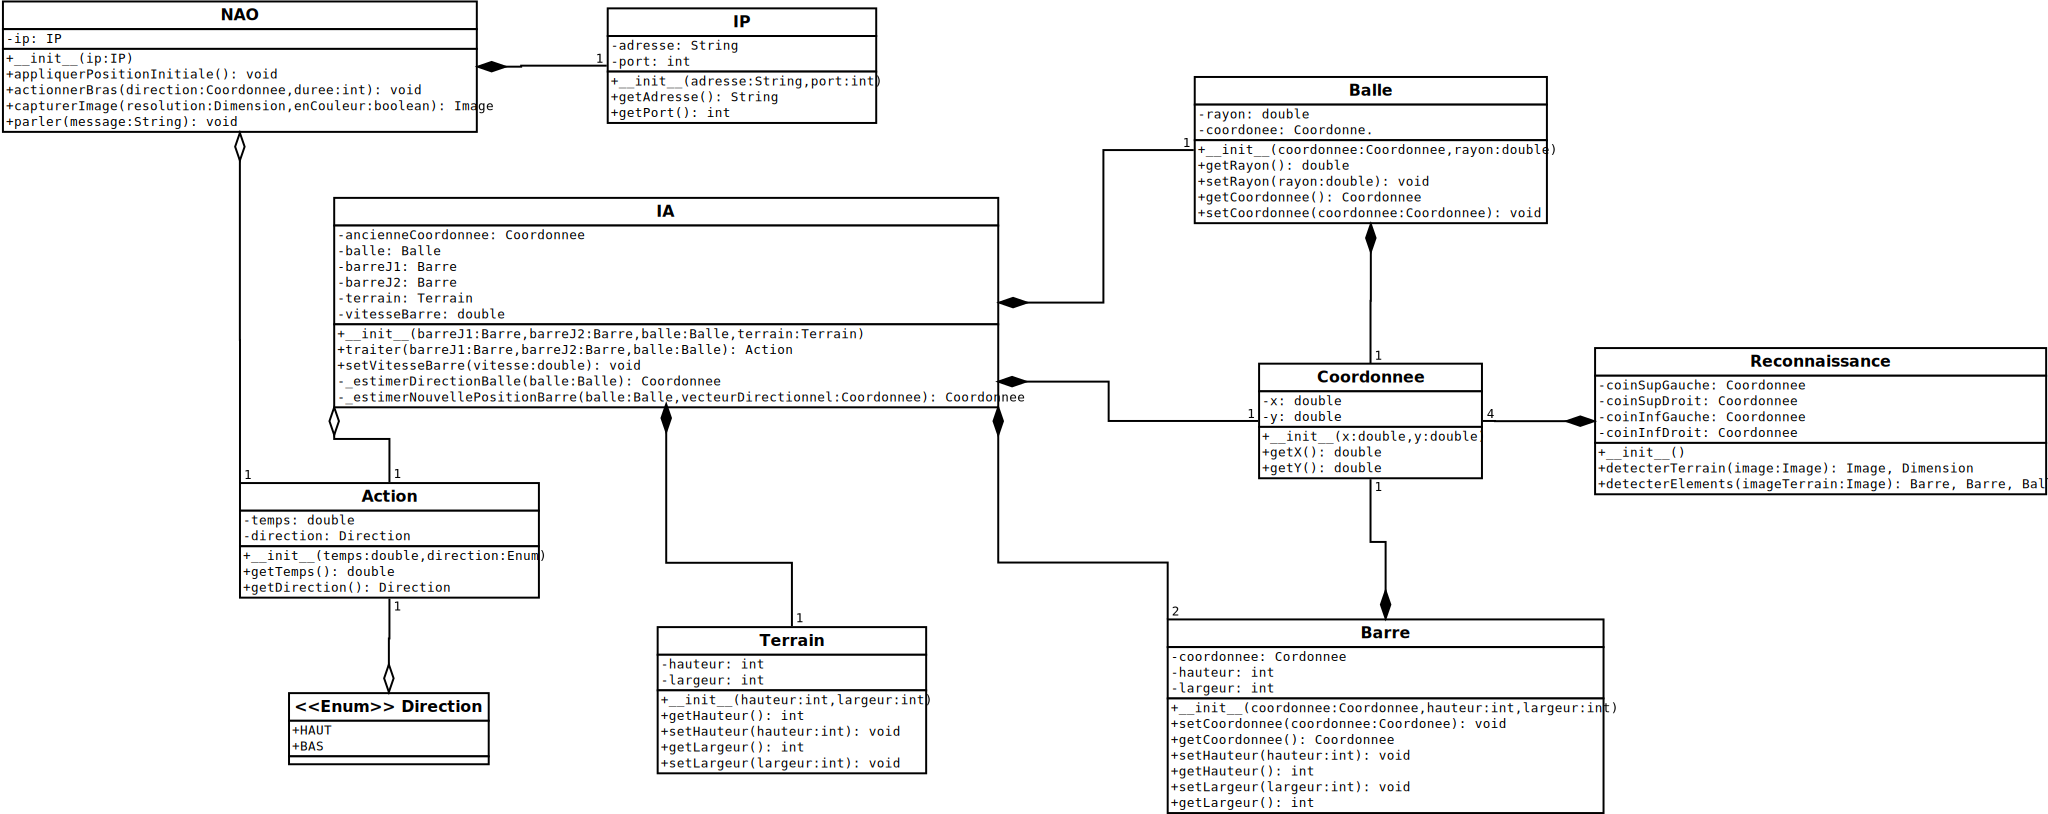
\includegraphics[angle=90, height=18cm, width=\textwidth]{Images/DiagrammeDeClasses.png}
  \end{figure}

\newpage

\section{Diagramme de séquence}
\label{sec:Diagramme de séquence}
  \begin{figure}[!h]
    \caption{Diagramme de séquence}
    \centering
    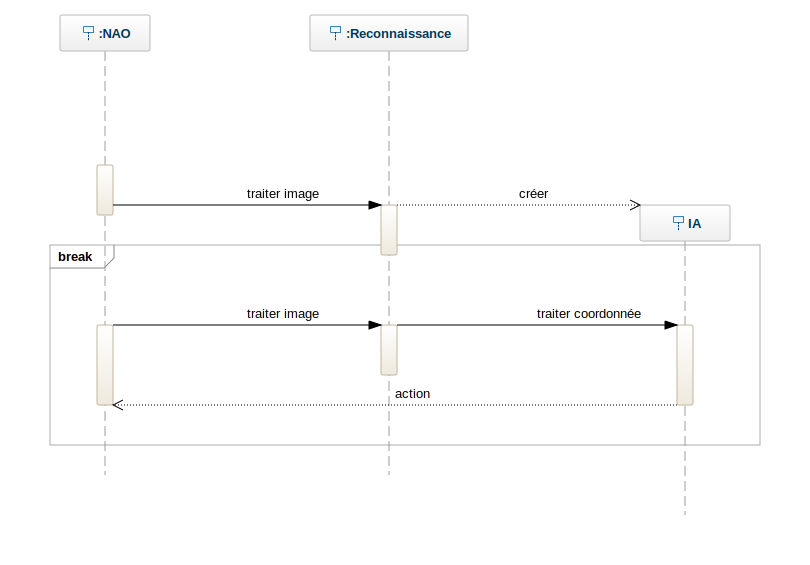
\includegraphics[width=\textwidth]{Images/DiagrammeDeSequence.png}
  \end{figure}



\end{document}
